\section{Inverse Abbildungen und inverse Matrizen}
\subsection{Begriffe und Formeln}
\begin{LA}
{Invertierbare Abbildung}{Inverse}
Sei 
\[
A = \begin{pmatrix} 3 & 16 \\ 1 & 4 \end{pmatrix}
\]
die Matrix einer linearen Abbildung \( f \) und 
\[
B = \begin{pmatrix} -1 & 4 \\ \frac{1}{4} & -\frac{3}{4} \end{pmatrix}
\]
jene von \( g \). Weiter sei 
\[
\vec{v} = \begin{pmatrix} x \\ y \end{pmatrix}
\]
ein beliebiger Vektor.

\begin{enumerate}
    \item Berechnen Sie \( \vec{w} = f(\vec{v}) \).
    \item Berechnen Sie nun \( g(\vec{w}) \).
    \item Berechnen Sie das Matrix-Produkt \( B \cdot A \).
\end{enumerate}
\end{LA}
\clearpage
\begin{LA}{nicht invertierbare Abbildung}{keineInverse}
Offenbar macht in \Cref{LA:Inverse} die Matrix $B$ die Wirkung von $A$ rückgängig. Betrachten Sie nun die Matrix
$$C = \begin{pmatrix}
    1&2 \\3&6
\end{pmatrix} $$

\begin{enumerate}
    \item Berechnen Sie $C\cdot\begin{pmatrix}
        2\\0
    \end{pmatrix}$ und $C\cdot\begin{pmatrix}
        0\\1
    \end{pmatrix}$.
    \item Berechnen Sie allgemein $C\cdot\begin{pmatrix}
        x\\y
    \end{pmatrix}$ und begründen Sie, wieso es keinen Vektor $\vec{v}$ gibt, mit der Eigenschaft, dass $C\cdot\vec{v} = \begin{pmatrix}
        1 \\2
    \end{pmatrix}$ ist.
    \item Geben Sie zwei Gründe an, wieso es keine Matrix gibt, welche die Wirkung von $C$ rückgängig macht.
\end{enumerate}
\end{LA}


















\clearpage
In der \Cref{LA:Inverse} haben Sie zwei zueinander inverse Abbildungen betrachtet. In diesem Kapitel wird genau definiert, was man unter einer inversen Abbildung versteht, und wir werden eine Formel angeben, mit der man die Inverse einer linearen Abbildung bestimmen kann.

\begin{definition}
    {Identität und Einheitsmatrix}{}
    Die lineare Abbildung mit der Eigenschaft, dass jeder Vektor auf sich selbst abgebildet wird, nennt man die \textbf{Identitätsabbildung}.  

\textbf{Notation:} \( \text{id} \), also  
\[
\text{id}(\vec{v}) = \vec{v} \quad \text{für alle Vektoren } \vec{v}.
\]

Die Abbildungsmatrix der Identitätsabbildung heisst \textbf{Einheitsmatrix}.  

In \( \mathbb{R}^2 \) gilt:
\[
E = \begin{pmatrix} 1 & 0 \\ 0 & 1 \end{pmatrix}.
\]
% In \( \mathbb{R}^3 \) gilt:

% \[
% E = \begin{pmatrix} 1 & 0 & 0 \\ 0 & 1 & 0 \\ 0 & 0 & 1 \end{pmatrix}.
% \]
\end{definition}
Die Identitätsabbildung ist das \textbf{neutrale Element} bezüglich der Komposition von Abbildungen. Für jede Abbildung \( f \) gilt:
\[
f \circ \text{id} = \text{id} \circ f = f
\]
Analog ist die Matrix \( E \) das \textbf{neutrale Element} bezüglich der Matrixmultiplikation. Für jede andere Matrix \( A \) gilt:
\[
A \cdot E = E \cdot A = A
\]

\begin{definition}
    {Inverse Abbildung und inverse Matrix}{}
    Seien \( f \) und \( f^{-1} \) zwei lineare Abbildungen mit der Eigenschaft:
    \[
    f \circ f^{-1} = \text{id}
    \]
    Dann nennt man \( f^{-1} \) die \textbf{inverse Abbildung} zu \( f \).

    \textbf{Analog:}  

    Seien \( A \) und \( A^{-1} \) zwei Matrizen mit der Eigenschaft, dass
    \[
    A \cdot A^{-1} = E.
    \]
    Dann nennt man \( A^{-1} \) die \textbf{inverse Matrix} zu \( A \).
\end{definition}

\begin{bsp}
    {}{}
    Die folgenden Matrizen sind invers zueinander:
    \[
    A = \begin{pmatrix} 3 & 16 \\ 1 & 4 \end{pmatrix}, \quad
    B = \begin{pmatrix} -1 & 4 \\ \frac{1}{4} & -\frac{3}{4} \end{pmatrix}
    \]
    Es gilt nämlich:
    \[
    A \cdot B =
    \begin{pmatrix} 
    3 \cdot (-1) + 16 \cdot \frac{1}{4} & 3 \cdot 4 + 16 \cdot \left(-\frac{3}{4} \right) \\ 
    1 \cdot (-1) + 4 \cdot \frac{1}{4} & 1 \cdot 4 + 4 \cdot \left(-\frac{3}{4} \right)
    \end{pmatrix}
     =
    \begin{pmatrix} 
    -3 + 4 & 12 - 12 \\ 
    -1 + 1 & 4 - 3
    \end{pmatrix}
    =
    \begin{pmatrix} 1 & 0 \\ 0 & 1 \end{pmatrix}
    \]

\end{bsp}
\clearpage
% \begin{bsp}
%     {}{}
%     Gegeben ist die Matrix:

% \[
% A =
% \begin{pmatrix} a_{11} & a_{12} \\ a_{21} & a_{22} \end{pmatrix}.
% \]

% Zeigen Sie, dass die Matrix:

% \[
% B = \frac{1}{a_{11} a_{22} - a_{12} a_{21}}
% \begin{pmatrix} a_{22} & -a_{12} \\ -a_{21} & a_{11} \end{pmatrix}
% \]

% die Inverse von \( A \) ist.

% \vspace*{10cm}

% \end{bsp}

\begin{bsp}
    {Formel für die Inverse}{}
        Gegeben ist die Matrix:
\[
A =
\begin{pmatrix} a & b \\ c & d \end{pmatrix}.
\]
Gesucht ist deren inverse Matrix 
\[
A^{-1} =
\begin{pmatrix} w & x \\ y & z \end{pmatrix}.
\]

\vspace*{18cm}
\end{bsp}
\clearpage



\begin{definition}
    {Determinante}{}
    Sei $$A= \begin{pmatrix}
        a & b \\ c & d
    \end{pmatrix}$$
    Die Zahl 
    $$ \det(A) = ad-bc$$
    nennt man die \emph{Determinante} der Matrix $A$.
\end{definition}

\begin{satz}
    {Berechnung der inversen Matrix}{}
    Sei \( A \) die Matrix:
    $$A= \begin{pmatrix}
        a & b \\ c & d
    \end{pmatrix}$$
    mit Determinante:
    $$ \det(A) = ad-bc$$
    Falls \( \det(A) \neq 0 \) gilt:
    \[
    A^{-1} = \phantom{\frac{1}{\det(A)}
    \begin{pmatrix} a_{22} & -a_{12} \\ -a_{21} & a_{11} \end{pmatrix}}
    \]

    Falls \( \det(A) = 0 \) hat die Matrix \( A \) keine Inverse.

\end{satz}
\begin{bsp}
    {}{}
    Die Matrix 
\[
A =
\begin{pmatrix} 1 & 2 \\ 3 & 4 \end{pmatrix}
\]
ist invertierbar, denn 

\[
\det(A) = 1 \cdot 4 - 2 \cdot 3 = -2.
\]

Es gilt:

\[
A^{-1} = \frac{1}{-2} 
\begin{pmatrix} 4 & -2 \\ -3 & 1 \end{pmatrix}
=
\begin{pmatrix} -2 & 1 \\ \frac{3}{2} & -\frac{1}{2} \end{pmatrix}
\]

\end{bsp}

\begin{bsp}
    {Nicht-invertierbare Matrix}{}
    Die Matrix $B=\begin{pmatrix}
        1&2 \\3&6
    \end{pmatrix}$ ist nicht invertierbar, denn
    $$\det B = 1\cdot 6 - 3\cdot 2 = 0$$
    Die entsprechende lineare Abbildung ist auch nicht invertierbar, denn
    $$ B\begin{pmatrix}
        2 \\0 
    \end{pmatrix}  = \begin{pmatrix}
        2 \\6
    \end{pmatrix} \qquad \text{und} \qquad B\begin{pmatrix}
        0 \\1 
    \end{pmatrix} = \begin{pmatrix}
        2 \\6
    \end{pmatrix},$$
    womit die Abbildung nicht injektiv ist (surjektiv ist sie auch nicht, siehe \Cref{LA:keineInverse}). 
\end{bsp}
\pagebreak
\begin{ueb}
    {}{}
    \begin{enumerate}
        
    \item Gegeben ist die Matrix der linearen Abbildung \( f \):

    \[
    A = \begin{pmatrix}
    3 & 2 \\
    5 & 4
    \end{pmatrix}
    \]
    
    \begin{enumerate}
      \item Bestimmen Sie die Matrix der inversen Abbildung \( f^{-1} \).
      \item Bestimmen Sie das Urbild des Vektors 
      \[
      \vec{v} = \begin{pmatrix}
      -10 \\
      8
      \end{pmatrix},
      \]
      d.\,h. denjenigen Vektor, der durch \( f \) auf \( \vec{v} \) abgebildet wird.
    \end{enumerate}

    \item Die Abbildung \( f \) ist die Spiegelung an der Geraden \( y = x \),  
    die Abbildung \( g \) ist die Drehung um den Ursprung \( O \) um \( 30^\circ \) gegen den Uhrzeigersinn.
    
    \begin{enumerate}
      \item Ermitteln Sie die Matrix \( A_f \) der Abbildung \( f \). Welche geometrische Bedeutung hat diese Matrix?
      \item Ermitteln Sie die Matrix \( A_g \) der Abbildung \( g \). Welche geometrische Bedeutung hat diese Matrix?
      \item Berechnen Sie \( A_f^{-1} \) und \( A_g^{-1} \).
      \item Zeigen Sie, dass $(A_f \cdot A_g)^{-1} = A_g^{-1} \cdot A_f^{-1}$ gilt. Geben Sie eine geometrische Deutung an.
      \item Bestimmen Sie die Matrix \( A_h \) einer Abbildung \( h \), sodass gilt:
      \[
      h \circ f = g
      \]
      \item Bestimmen Sie die Matrix \( A_h \) einer Abbildung \( h \), sodass gilt:
      \[
      f \circ h = g
      \]
    %   \textit{Hinweis: Multiplizieren Sie die Gleichung von links mit der Inversen von \( A_f \), also \( A_f^{-1} \).}
    \end{enumerate}
    \item Die Matrix einer Drehung gegen den Uhrzeigersin um den Ursprung um den Winkel \( \alpha \) ist gegeben durch:
    \[
    A_\alpha = \begin{pmatrix}
    \cos(\alpha) & -\sin(\alpha) \\
    \sin(\alpha) & \cos(\alpha)
    \end{pmatrix}
    \]
    Überlegen Sie sich, wie die Matrix der Inversen Abbildung aussieht. Berechnen Sie die Inverse der Matrix \( A_\alpha \) und überprüfen Sie Ihre Überlegung.
    \end{enumerate}
\end{ueb}

\begin{ueb}
    {Programmieraufgabe}{}
    Ergänzen Sie die Klasse \lstinline|matrix2x2| um die Methoden
    \begin{itemize}
        \item \lstinline|det(self)| für die Berechnung der Determinante einer Matrix.
        \item \lstinline|inv(self)| für die Berechnung der Inversen einer Matrix.
    \end{itemize}
\end{ueb}


\clearpage
\emph{Lösungen}
\begin{enumerate}

    \item
    \begin{enumerate}
      \item \( A^{-1} = \begin{pmatrix} 2 & -1 \\ -5/2 & 3/2 \end{pmatrix} \)
      \item \( \vec{u} = \begin{pmatrix} -28\\ 37 \end{pmatrix} \)
    \end{enumerate}
  
    \item
    \begin{enumerate}
      \item \( A_f = \begin{pmatrix} 0 & 1 \\ 1 & 0 \end{pmatrix} \)
      \item \( A_g = \begin{pmatrix} \cos(30^\circ) & -\sin(30^\circ) \\ \sin(30^\circ) & \cos(30^\circ) \end{pmatrix}
              = \begin{pmatrix} \frac{\sqrt{3}}{2} & -\frac{1}{2} \\ \frac{1}{2} & \frac{\sqrt{3}}{2} \end{pmatrix} \)
      \item \( A_f^{-1} = A_f = \begin{pmatrix} 0 & 1 \\ 1 & 0 \end{pmatrix} \),
            \quad
            \( A_g^{-1} = \begin{pmatrix} \frac{\sqrt{3}}{2} & \frac{1}{2} \\ -\frac{1}{2} & \frac{\sqrt{3}}{2} \end{pmatrix} \)
      \item \dots
        \item \( A_h = A_g \cdot A_f^{-1} = \begin{pmatrix} -\frac{1}{2} & \frac{\sqrt{3}}{2} \\ \frac{\sqrt{3}}{2} & \frac{1}{2} \end{pmatrix} \)
      \item \( A_h = A_f^{-1} \cdot A_g =  \begin{pmatrix} \frac{1}{2} & \frac{\sqrt{3}}{2} \\ \frac{\sqrt{3}}{2} & -\frac{1}{2} \end{pmatrix} \)
    \end{enumerate}
    \item $$ A^{-1} = \begin{pmatrix}
        \cos(-\alpha) & -\sin(-\alpha) \\
        \sin(-\alpha) & \cos(-\alpha)
    \end{pmatrix} = \begin{pmatrix}
        \cos(\alpha) & \sin(\alpha) \\
        -\sin(\alpha) & \cos(\alpha)
    \end{pmatrix}$$
  
  \end{enumerate}

  \clearpage






























  \subsection{Geometrische Bedeutung der Determinante}
  \begin{LA}
      {Geometrische Bedeutung der Determinante}{determinanteUndFläche}
      In dieser Aufgabe geht es um die geometrische Bedeutung der Determinante einer Matrix.

      Betrachten Sie dazu eine lineare Abbildung \( f \) mit der Abbildungsmatrix
      \[
      A = \begin{pmatrix}
      a_{11} & a_{12}  \\
      a_{21} & a_{22}
      \end{pmatrix}.
      \]
      
      Die Basisvektoren
      \[
      \vec{e}_1 = \begin{pmatrix} 1 \\ 0 \end{pmatrix}, \quad
      \vec{e}_2 = \begin{pmatrix} 0 \\ 1 \end{pmatrix}
      \]
      spannen ein Quadrat mit dem Flächeninhalt \( I = 1 \) auf.

      Unter der Abbildung $f$ wird das Quadrat in ein Viereck abgebildet. Im Folgenden soll der Flächeninhalt $I'$ dieses Vierecks berechnet werden. 
      
      \begin{enumerate}
        \item Wieso ist das Bild des Einheitsquadrates unter der Abbildung $f$ ein Parallelogramm, dessen Ecken die folgenden Koordinaten haben?
        \begin{center}
            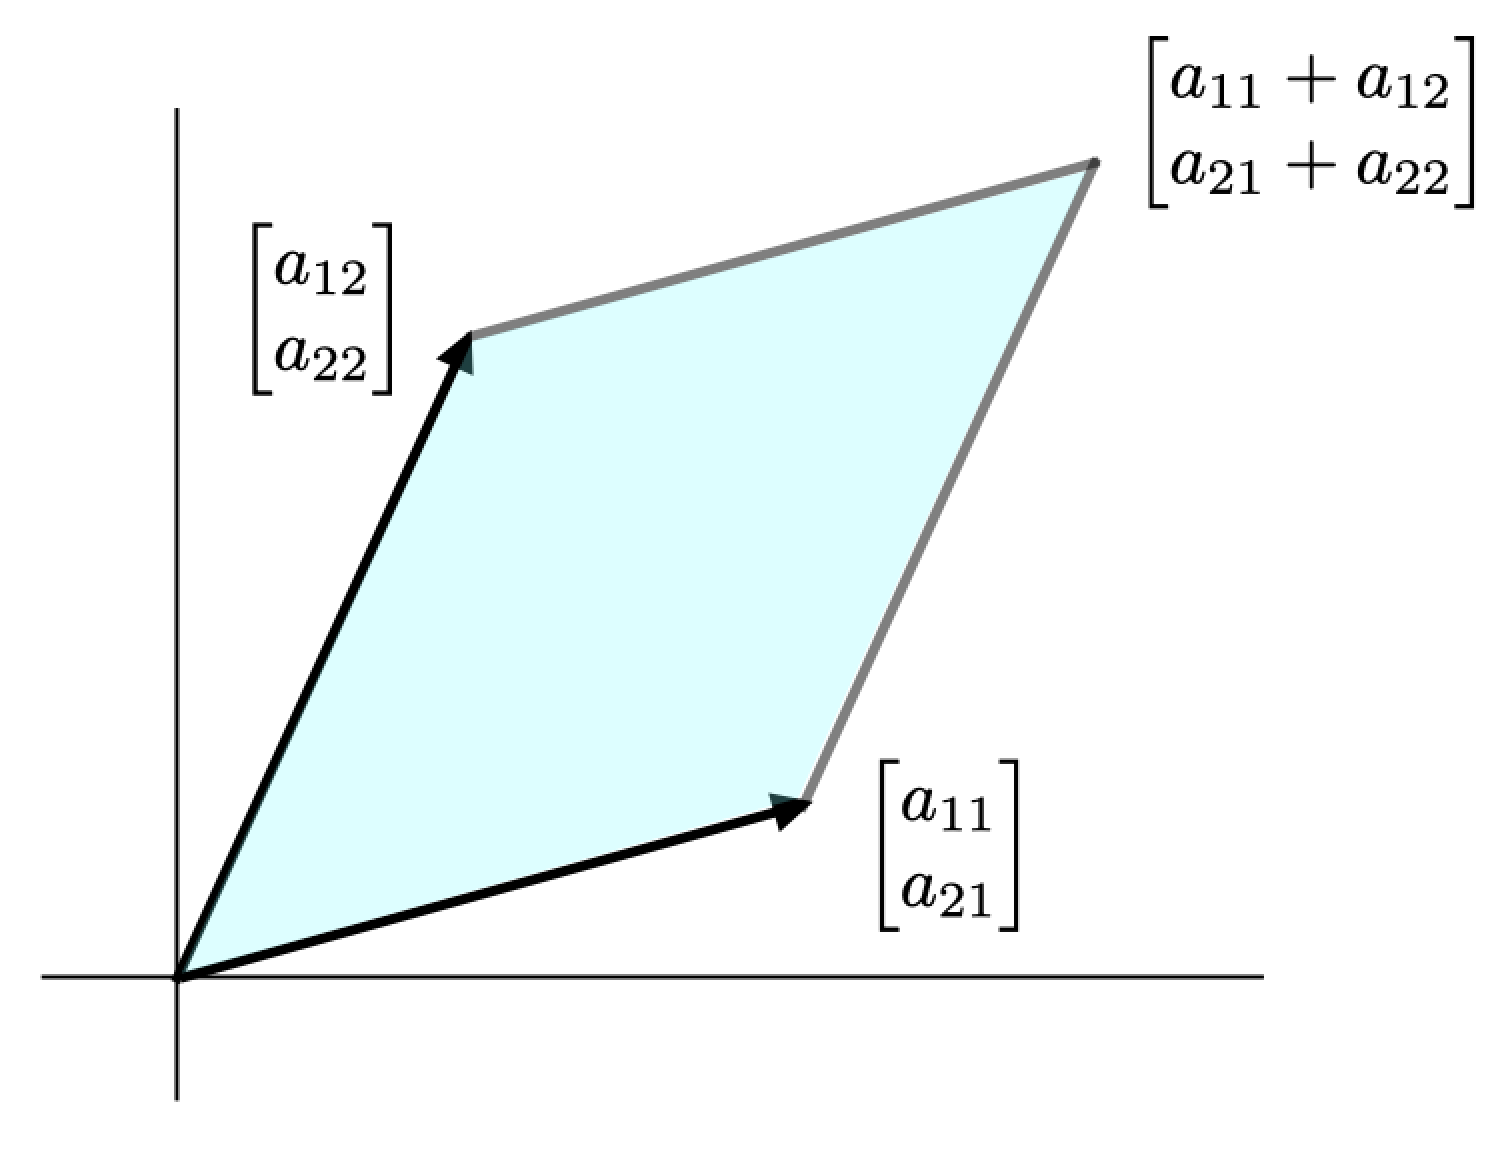
\includegraphics[width = 0.4\textwidth]{media/determinateFlaeche1.png}
        \end{center}
        \item Welchen Flächeninhalt \( I' \) hat das Parallelogramm? Nutzen Sie die folgende Hilfsfigur:
        \begin{center}
            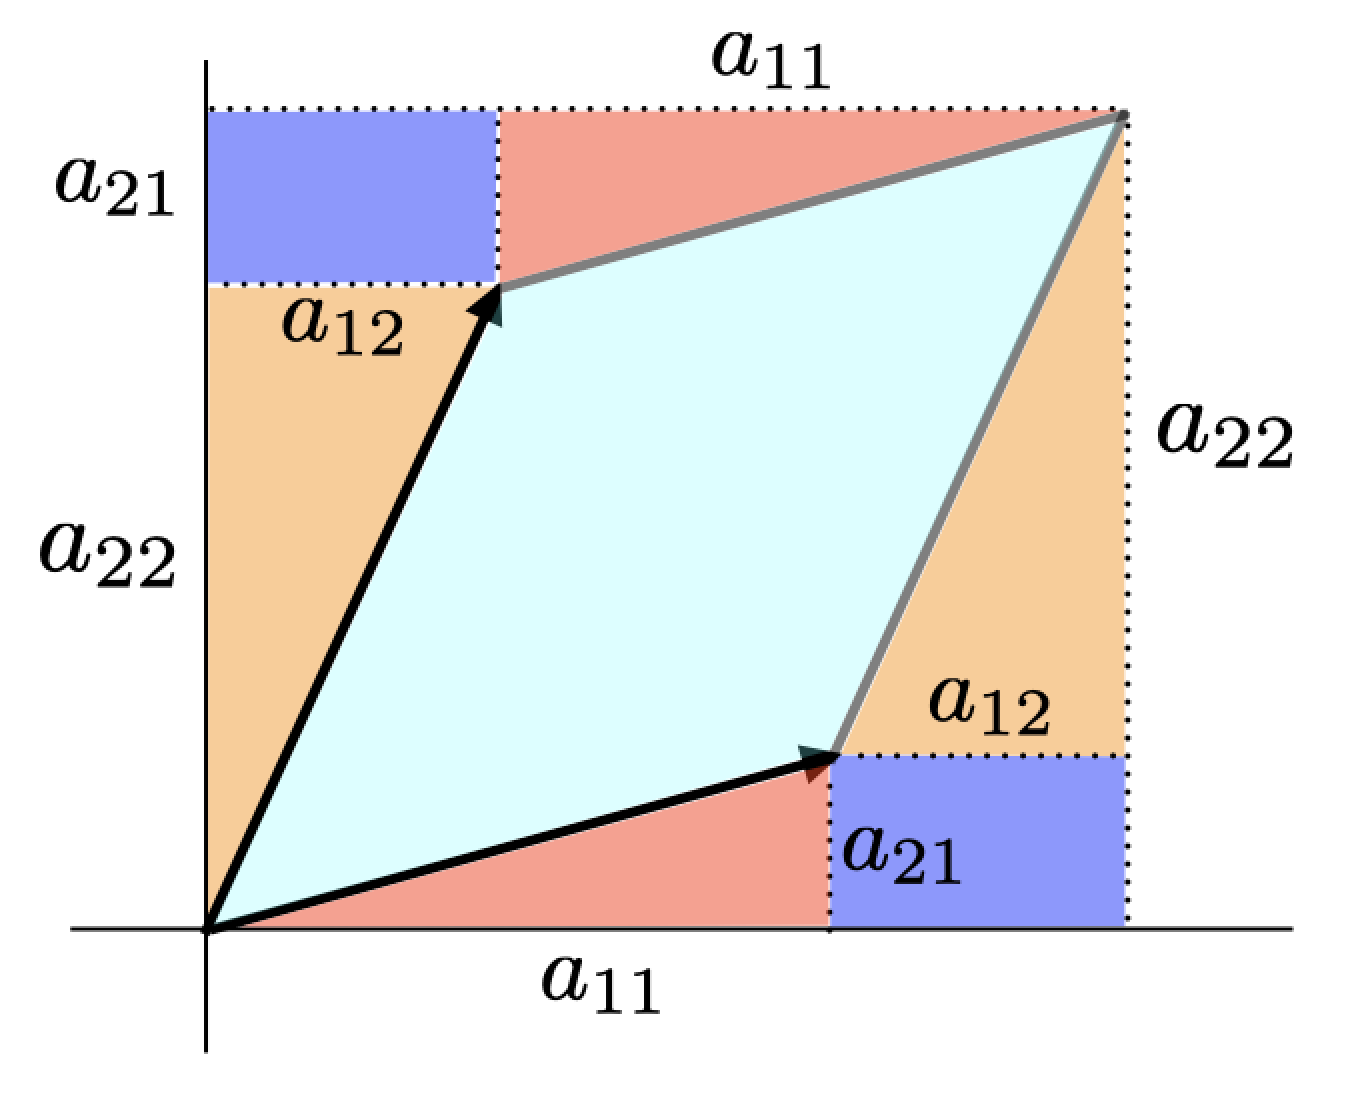
\includegraphics[width = 0.4\textwidth]{media/determinanteFlaeche2.png}
        \end{center}
      \end{enumerate}
      
  \end{LA}
  \clearpage
  Die Erkenntnisse aus \Cref{LA:determinanteUndFläche} gelten aufgrund der Linearität nicht nur für das Einheitsquadrat:
  \begin{satz}
    {Bedeutung der Determinante}{}
    Sei $f$ eine lineare Abbildung mit der Abbildungsmatrix $A$. Wird eine Figur mit dem Flächeninhalt $I$ abgebildet so hat die Bildfigur den Flächeninhalt

    $$ I' = |\det(A)| \cdot I$$
  \end{satz}

  \begin{ueb}
    {}{}
    \begin{enumerate}
        \item Welchen Wert hat die Determinante der Abbildung aufgrund der geometrischen Interpretation? Überprüfe die Vermutung, indem du die zur Abbildung passende Matrix bestimmst und deren Determinante berechnest
         \begin{enumerate}
            \item Drehung um den Ursprung um den Winkel \( \alpha \).
            \item Zentrische Streckung um den Faktor 5 mit Zentrum im Ursprung. 
            \item Projektion auf die \( y \)-Achse in Richtung des Vektors \( \vec{v} = \begin{pmatrix} 2 \\ 5 \end{pmatrix} \)
          \end{enumerate}
        \item Seien $A$ und $B$ $2\times2$-Matrizen und $\lambda\in\R$ eine Zahl. Welche Beziehung besteht zwischen 
        \begin{enumerate}
            \item $\det(A)$ und $\det(\lambda\cdot A)$?
            \item $\det(A), \det(B)$ und $\det(AB)$?
        \end{enumerate}
        Beweise die Vermutungen mit einer Rechnung.
    \end{enumerate}
  \end{ueb}
  

























  \clearpage
  \subsection{Lineare Gleichungssysteme und Matrizen}

Matrizen haben viel mit linearen Gleichungssystemen zu tun. Tatsächlich kann man jedes lineare Gleichungssystem mithilfe von Matrizen beschreiben und auch lösen.

Betrachten Sie das folgende Beispiel:

\begin{bsp}
    {Gleichungssystem in Matrixform}{}

\[
\begin{cases}
2x + 2y = -2 \\
5x + 6y = 6
\end{cases}
\]

Dieses Gleichungssystem kann auch in Matrixform geschrieben werden:

\vspace*{15cm}

% \[
% \begin{pmatrix}
% 2 & 2 \\
% 5 & 6
% \end{pmatrix}
% \cdot
% \begin{pmatrix}
% x \\
% y
% \end{pmatrix}
% =
% \begin{pmatrix}
% -2 \\
% 6
% \end{pmatrix}
% \]

% Unter diesem Blickwinkel wird nach einem Vektor $\begin{pmatrix}
%     x \\
%     y
%     \end{pmatrix}$ gesucht, der auf den Vektor $\begin{pmatrix}
%         -2 \\
%         6
%         \end{pmatrix}$ abgebildet wird. Für diese Fragestellung kennen wir bereits einen Lösungsweg:

% Die Inverse der Matrix \( A = \begin{pmatrix} 2 & 2 \\ 5 & 6 \end{pmatrix} \) ist:

% \[
% A^{-1} = \frac{1}{2} \begin{pmatrix} 6 & -2 \\ -5 & 2 \end{pmatrix}
% \]

% Daraus folgt:

% \[
% \begin{pmatrix}
% x \\
% y
% \end{pmatrix}
% =
% A^{-1} \cdot
% \begin{pmatrix}
% -2 \\
% 6
% \end{pmatrix}
% =
% \begin{pmatrix}
% -12 \\
% 11
% \end{pmatrix}
% \]

% Das Gleichungssystem hat also die Lösung \( x = -12 \), \( y = 11 \).
\end{bsp}
\clearpage
\begin{satz}
    {Matrizen und lineare Gleichungssysteme}{}
    Für das lineare Gleichungssystem
\[
\begin{cases}
a_{11}x + a_{12}y = b_1 \\
a_{21}x + a_{22}y = b_2
\end{cases}
\]
und die zugehörige Koeffizientenmatrix
\[
A = \begin{pmatrix}
a_{11} & a_{12} \\
a_{21} & a_{22}
\end{pmatrix}
\]
gilt:

\begin{itemize}
  \item Falls \( \det(A) \neq 0 \), so hat das Gleichungssystem genau eine Lösung, nämlich:
  \[
  \begin{pmatrix}
  x \\
  y
  \end{pmatrix}
  = A^{-1} \cdot
  \begin{pmatrix}
  b_1 \\
  b_2
  \end{pmatrix}
  \]
  
  \item Falls \( \det(A) = 0 \), so hat das Gleichungssystem entweder keine Lösung oder unendlich viele Lösungen.
\end{itemize}
\end{satz}
\paragraph{Bemerkung:}
Diese Lösungsmethode kann auch verwendet werden, um lineare Gleichungssysteme mit drei und mehr Unbekannten zu lösen (vorausgesetzt, es liegen entsprechend viele Gleichungen vor). 
Allerdings ist bereits ab drei Unbekannten der Aufwand zur Ermittlung der inversen Matrix so gross, dass sich die Lösung mit anderen Methoden — zum Beispiel dem Gauss-Verfahren — effizienter finden lässt.

\begin{ueb}
    {}{}

\begin{enumerate}
    \item Lösen Sie die folgenden Gleichungssysteme mit Hilfe der inversen Matrix:
    \begin{enumerate}
      \item
      \[
      \begin{cases}
      3x + 2y = -2 \\
      7x + 5y = 3
      \end{cases}
      \]
      \item
      \[
      \begin{cases}
      x + y = 26 \\
      x - y = 8
      \end{cases}
      \]
      \item
      \[
      \begin{cases}
      3x + 4y = 24 \\
      -x + 5y = 11
      \end{cases}
      \]
      \item
      \[
      \begin{cases}
      8x + 5y - 7 = 0 \\
      4x + 3y - 1 = 0
      \end{cases}
      \]
      \item
      \[
      \begin{cases}
      -4x + 6y = 5 \\
      6x - 9y = -8
      \end{cases}
      \]
      \item
      \[
      \begin{cases}
      -4x + 6y = 5 \\
      6x - 9y = -7.5
      \end{cases}
      \]
    \end{enumerate}
  
    \item Für welche Werte des Parameters besitzt das Gleichungssystem eine eindeutige Lösung?\\
    Begründen Sie, indem Sie die Determinante der entsprechenden Matrix untersuchen.
    \begin{enumerate}
      \item
      \[
      \begin{cases}
      ax + y = 5 \\
      x - y = -8
      \end{cases}
      \]
      \item
      \[
      \begin{cases}
      bx + by = 5 \\
      6x + by = -8
      \end{cases}
      \]
      \item
      \[
      \begin{cases}
      3x + 3cy = 5 \\
      cx + x + 3y = -8
      \end{cases}
      \]
    \end{enumerate}
  \end{enumerate}
  
\end{ueb}
\clearpage
\emph{Lösungen}

\begin{enumerate}
    \item Lösungen der Gleichungssysteme mit der inversen Matrix:
    \begin{enumerate}
      \item \( x = -16, \quad y = 23 \)
      \item \( x = 17, \quad y = 9 \)
      \item \( x = 4, \quad y = 3 \)
      \item \( x = 4, \quad y = -5 \)
      \item Keine Lösung .
      \item Unendlich viele Lösungen  
      Parametrisierte Lösungsmenge:
      \[
      \begin{pmatrix}
      x \\
      y
      \end{pmatrix}
      =
      \begin{pmatrix}
      -5 \\
      -\frac{5}{2}
      \end{pmatrix}
      +
      t \cdot
      \begin{pmatrix}
      \frac{3}{2} \\
      1
      \end{pmatrix},
      \quad t \in \mathbb{R}
      \]
    \end{enumerate}
    
  \item Eindeutige Lösbarkeit in Abhängigkeit vom Parameter:
  \begin{enumerate}
    \item Eindeutig lösbar für \( a \neq 1 \)
    \item Eindeutig lösbar für \( b \neq 0 \) und $b\neq 6$
    \item Eindeutig lösbar für \( c \neq -\frac{1}{2} \pm \frac{\sqrt{13}}{2} \)
  \end{enumerate}
  \end{enumerate}